\documentclass[conference]{IEEEtran}
\IEEEoverridecommandlockouts
% Template version as of 6/27/2024 (IEEEtran)

\usepackage{cite}
\usepackage{amsmath,amssymb,amsfonts}
\usepackage{algorithmic}
\usepackage{graphicx}
\usepackage{textcomp}
\usepackage{xcolor}
\usepackage{url}
\usepackage{tikz}
\usetikzlibrary{arrows.meta,positioning,shapes.geometric,fit}
\usepackage{array}

\begin{document}

\title{Individual Report: Final Project}

\author{\IEEEauthorblockN{Cendong Lu}
\IEEEauthorblockA{\textit{Master of Information Technology} \\
\textit{The University of Auckland}\\
Auckland, New Zealand \\
clu518@aucklanduni.ac.nz}
}

\maketitle

\begin{abstract}
This report describes the design and implementation of a personal blogging system developed as a team project in the Master of Information Technology programme at the University of Auckland. The system provides user registration and session-based authentication, profile management with avatars, article creation and editing, commenting, and an administrative desktop client. The architecture follows a classic three-tier design: a SvelteKit web frontend, a Node.js/Express REST API backend, and an SQLite relational database, with a separate Java Swing admin application consuming the same API. My individual contributions focused on the user identity lifecycle across the stack (registration, login/logout, cookie sessions, profile editing, avatar upload and serving, and a Swing login client), and on an AI-assisted online research feature that searches external sources, fetches pages, and produces a cited summary for an article. The report highlights how the database schema, API design, and UI components fit together, the class topics applied, the additional technologies adopted, and lessons learned from feature-based module ownership and integration in a short delivery timeline.
\end{abstract}

\begin{IEEEkeywords}
SvelteKit, Express, SQLite, session cookie authentication, Java Swing, REST API, generative AI, software architecture
\end{IEEEkeywords}

\section{Introduction}
The project goal was to build a secure, usable personal blogging platform with both a web interface for end users and a desktop administration client. The system needed to support user management (including password security), article and media management, and a commenting system, while maintaining consistent access control and predictable API behaviour under a tight schedule. Our team adopted feature-module ownership (vertical slices) so each member implemented complete end-to-end functionality across frontend, backend, database, and Swing components. This report documents the overall design and my individual work in the authentication/profile module and an AI-based research companion module.

\section{System Design and Architecture}
\subsection{High-level architecture}
The system consists of four interacting parts:
\begin{itemize}
\item \textbf{Web frontend (SvelteKit)}: Presents pages for registration, login, profile editing, article browsing and reading, and interactive features (e.g., comments). It calls the backend via a REST API and relies on browser-managed cookies for session persistence.
\item \textbf{Backend (Node.js/Express)}: Implements REST endpoints, enforces authentication and authorization, validates inputs, and coordinates file uploads and AI tasks.
\item \textbf{Database (SQLite)}: Stores users, sessions, articles, comments, and image metadata with foreign keys and cascade rules to preserve referential integrity.
\item \textbf{Swing admin client (Java)}: A separate desktop application that authenticates as an admin user and calls admin endpoints to list users and manage accounts.
\end{itemize}

\begin{figure*}[t]
\centering
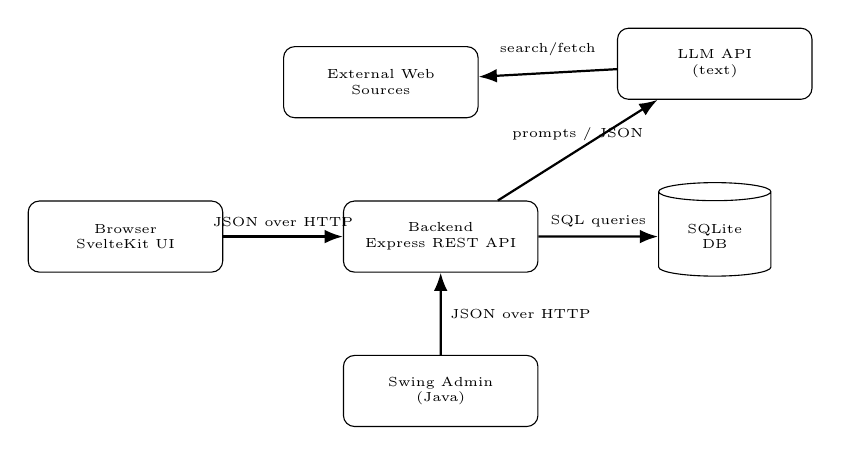
\begin{tikzpicture}[
  font=\tiny,  % change to \tiny, \scriptsize, \small, \normalsize, \large, etc.
  scale=0.95,
  transform shape,
  box/.style={draw, rounded corners, align=center, minimum width=2.6cm, minimum height=0.95cm},
  db/.style={draw, cylinder, shape border rotate=90, aspect=0.25, align=center, minimum height=1.25cm, minimum width=1.5cm},
  arr/.style={-Latex, thick}
]
  \node[box] (browser) {Browser\\SvelteKit UI};
  \node[box, right=1.6cm of browser] (api) {Backend\\Express REST API};
  \node[db, right=1.6cm of api] (sqlite) {SQLite\\DB};

  \node[box, above=1.1cm of api, xshift=-0.8cm] (web) {External Web\\Sources};
  \node[box, above=1.1cm of sqlite] (llm) {LLM API\\(text)};
  \node[box, below=1.1cm of api] (swing) {Swing Admin\\(Java)};

  \draw[arr] (browser) -- node[above]{JSON over HTTP} (api);
  \draw[arr] (api) -- node[above]{SQL queries} (sqlite);
  \draw[arr] (swing) -- node[right]{JSON over HTTP} (api);
  \draw[arr] (llm) -- node[pos=0.5, above=0.1cm]{search/fetch} (web);
  \draw[arr] (api) -- node[above]{prompts / JSON} (llm);
\end{tikzpicture}
\caption{High-level architecture showing web UI, backend API, database, Swing admin client, and AI research integrations.}
\label{fig:architecture}
\end{figure*}

\subsection{Data design}
The relational schema is centred on \texttt{USERS} and supports session-based authentication (\texttt{SESSIONS}), authored content (\texttt{ARTICLES}), engagement (\texttt{COMMENTS} with a self-referential parent relationship for nesting), and media (\texttt{IMAGES}). Deleting a user cascades deletion of their articles, comments, images, and sessions, which satisfies the requirement to remove a user and associated content.

\begin{figure*}[t]
\centering
% --- Fig.\ref{fig:erd}: Replace with your ER diagram image ---
% Put your image file (e.g.\ \texttt{er-diagram.pdf} or \texttt{fig2-erd.png}) in the same folder as this .tex file,
% or use a path such as \texttt{figures/er-diagram.pdf}. Then uncomment the line below and remove the placeholder.
%\includegraphics[width=\textwidth]{er-diagram}
% Placeholder (remove when you add the image):
\fbox{\parbox{0.9\textwidth}{\centering\vspace{4cm}\textit{[ER diagram: place your image file here; see comment above.]}\vspace{4cm}}}
\caption{Simplified ER diagram of the core tables and relationships.}
\label{fig:erd}
\end{figure*}

\subsection{Component fit and communication}
\subsubsection{Frontend composition}
The frontend uses SvelteKit file-based routing with page components for registration and profile management. A global Svelte store holds the currently authenticated user state. Form inputs are validated client-side for fast feedback (e.g., username pattern and password length), and then validated again server-side to protect the system.

\begin{figure}[htbp]
\centering
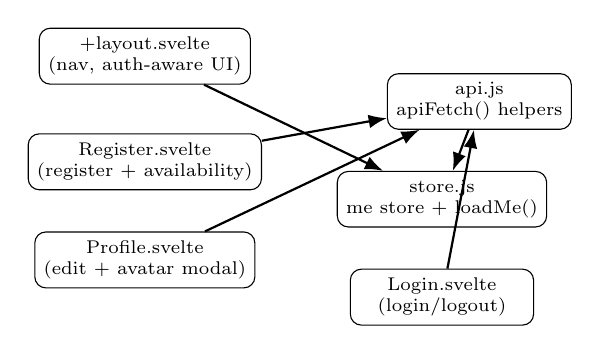
\begin{tikzpicture}[
  font=\scriptsize,
  scale=0.95,
  transform shape,
  comp/.style={draw, rounded corners, align=center, minimum width=2.45cm, minimum height=0.72cm},
  store/.style={draw, rounded corners, align=center, minimum width=2.45cm, minimum height=0.72cm},
  arr/.style={-Latex, thick}
]
  \node[comp] (layout) {+layout.svelte\\(nav, auth-aware UI)};
  \node[comp, below=0.65cm of layout] (register) {Register.svelte\\(register + availability)};
  \node[comp, below=0.55cm of register] (profile) {Profile.svelte\\(edit + avatar modal)};

  \node[store, right=1.0cm of register,yshift=-0.5cm] (meStore) {store.js\\me store + loadMe()};
  \node[comp, above=0.55cm of meStore,xshift=0.5cm] (apiFetch) {api.js\\apiFetch() helpers};
  \node[comp, below=0.55cm of meStore] (login) {Login.svelte\\(login/logout)};

  \draw[arr] (layout) -- (meStore);
  \draw[arr] (register) -- (apiFetch);
  \draw[arr] (login) -- (apiFetch);
  \draw[arr] (profile) -- (apiFetch);
  \draw[arr] (apiFetch) -- (meStore);
\end{tikzpicture}%
\caption{Auth/profile-related Svelte components and shared state.}
\label{fig:component}
\end{figure}

\subsubsection{Backend layering}
The backend separates concerns into route handlers (HTTP), middleware (authentication attachment and guards), and services (database operations and business rules). In particular, an \texttt{attachUser} middleware reads the \texttt{sid} cookie, verifies the session is unexpired, loads the user record, and attaches it to \texttt{req.user}. Downstream route handlers apply \texttt{requireAuth} to enforce login and \texttt{requireAdmin} to restrict admin endpoints. Cookie sessions are implemented with an \texttt{sid} cookie and a server-side \texttt{sessions} table. Session tokens are stored as SHA-256 hashes in the database rather than raw tokens to reduce damage if the database is compromised.

\subsubsection{Client--server protocols}
Most requests are JSON REST calls. Avatars and other images are served as image bytes. Authentication uses an HTTP-only cookie (SameSite=Lax) so the browser automatically sends the cookie with same-site requests while preventing JavaScript access to the cookie value.

\subsection{API design overview}
The API follows resource-oriented naming with consistent status codes and JSON error bodies. Table~\ref{tab:auth-api} summarizes the endpoints most relevant to my module (authentication, profile management, and avatars).

\begin{table}[htbp]
\caption{Authentication and profile API (selected endpoints)}
\label{tab:auth-api}
\centering
\renewcommand{\arraystretch}{1.15}
\begin{tabular}{|>{\raggedright\arraybackslash}p{1.0cm}|>{\raggedright\arraybackslash}p{3.8cm}|>{\raggedright\arraybackslash}p{0.9cm}|}
\hline
\textbf{Method} & \textbf{Path} & \textbf{Auth} \\
\hline
POST & \texttt{/api/users} & No \\
\hline
GET & {\tiny\texttt{/api/users/exists?username=...}} & No \\
\hline
POST & \texttt{/api/login} & No \\
\hline
POST & \texttt{/api/logout} & Optional \\
\hline
GET & \texttt{/api/me} & Yes \\
\hline
PATCH & \texttt{/api/users/me} & Yes \\
\hline
DELETE & \texttt{/api/users/me} & Yes \\
\hline
POST & \texttt{/api/users/me/avatar} & Yes \\
\hline
GET & \texttt{/api/users/:id/avatar} & No \\
\hline
\end{tabular}
\end{table}

\subsection{Targeted problems and solutions}
\paragraph{Preventing username collisions.}
The system provides both a live availability endpoint and a unique constraint in the database. The registration UI debounces checks to reduce server load and improve UX.

\paragraph{Password and session security.}
Passwords are stored only as bcrypt hashes. Sessions store only a hash of the session token and have a defined expiry window (one week) to reduce long-lived session risk.

\paragraph{Avatar usability without compromising simplicity.}
Users can select from predefined avatars (stored on the server) or upload a custom avatar image. The profile UI adds cache-busting query parameters so updated avatars appear immediately.

\section{Individual Contributions}
\subsection{Frontend contributions (SvelteKit)}
My main frontend work covered the registration and profile flows:
\begin{itemize}
\item \textbf{Registration UX}: Implemented username validation (\texttt{^[a-zA-Z0-9\_]\{3,20\}$}), password length checks (8--72 characters), and a debounced (300\,ms) availability check via \texttt{GET /api/users/exists?username=...}. Registration supports optional profile fields and avatar selection (predefined or upload).
\item \textbf{Custom avatar upload on registration}: When a user chooses upload mode, the UI creates the account, logs in to obtain a session cookie, and then uploads the avatar using multipart form data.
\item \textbf{Profile management}: Implemented profile editing and avatar switching (predefined vs uploaded) with a modal UI. Avatar display uses \texttt{/api/users/\{id\}/avatar} with a timestamp parameter to avoid stale browser caching.
\item \textbf{Auth state management}: Added a global store to load and cache the current user from \texttt{GET /api/me} on app startup or after profile changes.
\end{itemize}

\subsection{Backend contributions (Node.js/Express)}
My backend contributions implemented the user identity lifecycle and supported both the web app and Swing client:
\begin{itemize}
\item \textbf{Authentication endpoints}: Implemented \texttt{POST /api/login}, \texttt{POST /api/logout}, and \texttt{GET /api/me}. Login compares bcrypt hashes and sets an \texttt{sid} session cookie after creating a session record.
\item \textbf{User endpoints}: Implemented \texttt{POST /api/users} (register), \texttt{GET /api/users/exists} (availability), \texttt{PATCH /api/users/me} (profile update), and \texttt{DELETE /api/users/me} (account deletion).
\item \textbf{Avatar upload and serving}: Implemented \texttt{POST /api/users/me/avatar} using a server-side upload utility to store files under \texttt{uploads/avatars}. Implemented \texttt{GET /api/users/:id/avatar} to serve either the uploaded file or a predefined avatar.
\item \textbf{Session middleware and guards}: Implemented middleware to attach the authenticated user to the request by reading \texttt{sid} and looking up an unexpired session. Added \texttt{requireAuth} and \texttt{requireAdmin} guards for protected endpoints.
\end{itemize}

\begin{figure}[htbp]
\centering
\begin{tikzpicture}[
  font=\scriptsize,
  scale=0.95,
  transform shape,
  step/.style={draw, rounded corners, align=center, minimum width=2.5cm, minimum height=0.72cm},
  arr/.style={-Latex, thick}
]
  % Vertical layout to avoid clipping in narrow columns.
  \node[step] (s1) {Client\\POST /api/login\\(username,password)};
  \node[step, below=0.45cm of s1] (s2) {Server\\bcrypt compare\\create session row};
  \node[step, below=0.45cm of s2] (s3) {Response\\Set-Cookie: sid=...\\HttpOnly};
  \node[step, below=0.65cm of s3] (s4) {Later request\\Cookie: sid=...};
  \node[step, below=0.45cm of s4] (s5) {attachUser\\lookup sessions\\expires\_at check};
  \node[step, below=0.45cm of s5] (s6) {Route handler\\req.user present\\authorize};

  \draw[arr] (s1) -- (s2);
  \draw[arr] (s2) -- (s3);
  \draw[arr] (s4) -- (s5);
  \draw[arr] (s5) -- (s6);
\end{tikzpicture}%
\caption{Simplified login/session sequence used by both web and Swing clients.}
\label{fig:login-seq}
\end{figure}

\subsection{Design decisions in my module}
\paragraph{Cookie sessions instead of tokens in local storage.}
We used an HTTP-only cookie for session state rather than storing bearer tokens in frontend local storage. This reduces the risk of client-side script access to authentication credentials and makes browser requests naturally include session context. The backend therefore becomes the single place to enforce session expiry and to revoke sessions on logout or account deletion.

\paragraph{Hashing session tokens at rest.}
The session token stored in the \texttt{sid} cookie is treated as a secret. Only a SHA-256 hash is stored in the database, while the raw token remains only in the user's browser cookie. This choice reduces blast radius if session rows are leaked.

\paragraph{Predefined avatars plus upload.}
Predefined avatars provide a low-friction default that avoids file upload complexity for users. The upload option supports personalization while keeping implementation and moderation scope manageable (e.g., file size/type checks and storing uploads under a dedicated directory).

\subsection{Swing contributions (Java)}
To support administration, I implemented a reusable HTTP client and a login dialog:
\begin{itemize}
\item \textbf{HTTP client with cookie persistence}: The \texttt{HTTPClient} reads the \texttt{Set-Cookie} header on login, stores the cookie key-value, and attaches it as a \texttt{Cookie} header for later requests.
\item \textbf{Non-blocking login UI}: The \texttt{LoginDialog} performs network calls inside \texttt{SwingWorker} to avoid freezing the event dispatch thread, and exposes callbacks to notify the main admin app of login/logout state changes.
\end{itemize}

\subsection{AI research companion module}
In addition to authentication and profile management, I contributed an AI-assisted research feature designed to improve the reading experience on article pages. The implemented backend service follows this pipeline:
\begin{enumerate}
\item \textbf{Query generation}: Extracts a plain-text snippet from article HTML and uses a text-generation API to produce a short search query in strict JSON (6--12 words).
\item \textbf{Web search}: Calls a search tool with a configurable result limit (quick/standard/deep modes).
\item \textbf{Fetch and extract}: Fetches the top pages with timeouts and size caps, then extracts readable text.
\item \textbf{Summarization with citations}: Produces a 3--8 bullet Markdown summary, attaching source URLs inline to each bullet when possible and generating ``questions to verify'' when evidence is weak.
\item \textbf{Caching and status}: Stores status (\texttt{queued/running/ready/failed}), summary, sources, and expiry time in an \texttt{article\_research} table. Updates emit events so the UI can refresh at appropriate times.
\end{enumerate}
Key engineering concerns addressed include timeouts, limiting external requests, and ensuring the model does not invent URLs by constraining summarization to fetched sources.

\section{Topics from Class Used in the Project}
This project applied multiple topics covered in coursework:
\begin{itemize}
\item \textbf{System architecture}: tiered client--server design, separation of concerns, and module boundaries.
\item \textbf{Relational data modelling}: ER modelling, primary/foreign keys, uniqueness constraints, and cascade delete rules.
\item \textbf{REST API design}: consistent endpoint naming, HTTP methods, and status code conventions.
\item \textbf{Security fundamentals}: password hashing, session management, least privilege via middleware guards, and safe cookie settings (HttpOnly, SameSite).
\item \textbf{Concurrency and responsiveness}: background tasks in Swing (\texttt{SwingWorker}) and asynchronous I/O in Node.js.
\item \textbf{Software engineering practice}: feature-based ownership, integration planning, and incremental demos with a clear definition of done.
\end{itemize}

\section{Additional Topics and Technologies Not Taught in Class}
We adopted several technologies and patterns beyond core lecture content:
\begin{itemize}
\item \textbf{SvelteKit}: file-based routing, reactive stores, and component-driven UI composition.
\item \textbf{Multipart uploads}: using middleware to validate and persist image uploads, plus controlled static file serving patterns.
\item \textbf{AI tool orchestration}: using an LLM to generate structured outputs (strict JSON), chaining web search and fetch steps, and enforcing guardrails (timeouts, limits, citations).
\item \textbf{Caching with TTL}: storing derived AI outputs with expiry times to manage cost and latency.
\end{itemize}

\section{Generative AI Usage: Benefits and Drawbacks}
\subsection{How generative AI was used}
The project used generative AI in two main ways: (i) a research companion that searches external sources and summarizes them with citations for article readers, and (ii) an AI image workflow for generating article header images when users do not upload one. During development, AI assistants were also used as productivity tools for drafting boilerplate, clarifying library usage, and reviewing edge cases.

\subsection{Benefits}
The strongest benefits were development speed (especially for repetitive patterns), improved UX features that would otherwise be out of scope in the timeframe, and faster iteration on prompts and validation rules. For the research companion, AI enabled a concise, reader-oriented summary that could be updated as sources change.

\subsection{Drawbacks and mitigations}
Key drawbacks included hallucination risk, inconsistent output formatting, and security risks around fetching arbitrary URLs. We mitigated these by requiring strict JSON outputs, limiting the number of fetched pages, adding request timeouts and size caps, and ensuring citations are attached to summary bullets so the user can verify claims. Caching reduced cost and rate-limited repeated requests.

\section{Teamwork Lessons Learned}
\subsection{Benefits of feature-module ownership}
Vertical slice ownership reduced merge conflicts and made accountability clear. Each team member could deliver and demo a complete feature end-to-end, which improved confidence during integration. A shared ERD and API specification served as a single source of truth to reduce frontend--backend mismatches.

\subsection{Difficulties and how we addressed them}
The primary challenge was integration risk (e.g., authentication affecting articles and comments) under time pressure. We handled this by keeping integration points minimal, agreeing on consistent API shapes and error formats, and using early ``thin slice'' demos to detect mismatches. We also tracked risks such as scope creep and UI blocking (Swing) and used targeted mitigations such as prioritizing required features and moving network calls off the UI thread.

\section{Testing and Validation}
Given the short timeline, we relied on systematic manual testing aligned with the API contract and UI behaviours. For the authentication and profile module, key test cases included: registering with invalid usernames/passwords; verifying that username conflicts return a clear error (409 conflict) while the UI provides live feedback; confirming that login sets an \texttt{sid} cookie and that subsequent requests resolve \texttt{req.user}; ensuring logout removes the session; validating that deleting an account removes sessions and related content via cascade rules; and testing avatar upload failure modes (missing file, invalid type/size) without crashing the server. For Swing, repeated login/logout and user list refresh tests validated that network operations do not freeze the UI (by using \texttt{SwingWorker}).

\section{Limitations and Future Improvements}
Several improvements are straightforward extensions of the current design. First, CSRF protection could be strengthened by adding anti-CSRF tokens for state-changing requests in addition to SameSite cookie settings. Second, avatar and embedded media handling could be enhanced with stricter content-type verification, image resizing, and storage quotas. Third, the AI research companion should continue to harden safety boundaries (e.g., stricter SSRF protections and domain reputation filters) and improve transparency by showing timestamps and explicit disclaimers about AI uncertainty. Finally, broader automated tests (API-level and UI-level) would increase confidence for future iteration beyond the course timeframe.

\section{Conclusion}
The final system demonstrates a complete personal blogging workflow with secure session-based authentication, profile and avatar management, content and comments, and a Swing admin client. My contributions delivered the identity management module across the stack and an AI-assisted research companion feature with practical guardrails. The project reinforced the importance of clear API contracts, layered architecture, and disciplined scope management in a short timeline, while highlighting both the value and the limitations of AI-assisted development.


\end{document}